\documentclass[tikz,border=2pt]{standalone}
\usepackage[T1]{fontenc}
\usepackage{helvet,amsmath,amssymb,fix-cm}
\renewcommand{\familydefault}{\sfdefault}
\usetikzlibrary{arrows.meta,calc,positioning,fit,backgrounds,decorations.pathreplacing,shapes.geometric}
\definecolor{ink}{HTML}{243343}
\definecolor{physical}{HTML}{3478A3}
\definecolor{semantic}{HTML}{B27C26}
\definecolor{feasible}{HTML}{248679}
\definecolor{decode}{HTML}{75609D}
\definecolor{fault}{HTML}{BA5554}
\definecolor{muted}{HTML}{6F7D88}
\tikzset{
  every node/.style={font=\fontsize{9}{10.8}\selectfont,text=ink},
  edge/.style={-{Stealth[length=1.8mm,width=1.25mm]},line width=.6pt,draw=ink},
  param/.style={-{Stealth[length=1.7mm]},line width=.6pt,draw=decode,dashed},
  link/.style={line width=.8pt,draw=physical},
  reject/.style={line width=.7pt,draw=fault,dashed},
  panel/.style={rounded corners=2pt,draw=muted!45,line width=.45pt,fill=white},
  box/.style={rounded corners=2pt,draw=physical!70,line width=.55pt,fill=physical!6,align=center,inner sep=3pt},
  sem/.style={box,draw=semantic!70,fill=semantic!8},
  gate/.style={box,draw=feasible!70,fill=feasible!7},
  dec/.style={box,draw=decode!70,fill=decode!7},
  tinylabel/.style={font=\fontsize{8}{9.4}\selectfont},
  smalllabel/.style={font=\fontsize{8.5}{10}\selectfont},
  heading/.style={font=\bfseries\fontsize{10}{11.5}\selectfont,anchor=north west},
  dot/.style={circle,minimum size=.43cm,inner sep=0pt,draw=physical,fill=white,line width=.8pt,font=\bfseries\fontsize{9}{10}\selectfont},
  receiver/.pic={\draw[draw=physical,line width=.8pt] (0,0)--(0,.58) (-.17,0)--(.17,0) (-.15,.39)--(0,.58)--(.15,.39);
    \draw[draw=physical!70,line width=.55pt] (-.2,.56) arc[start angle=160,end angle=200,radius=.23];
    \draw[draw=physical!70,line width=.55pt] (.2,.40) arc[start angle=-20,end angle=20,radius=.23];},
}
\begin{document}
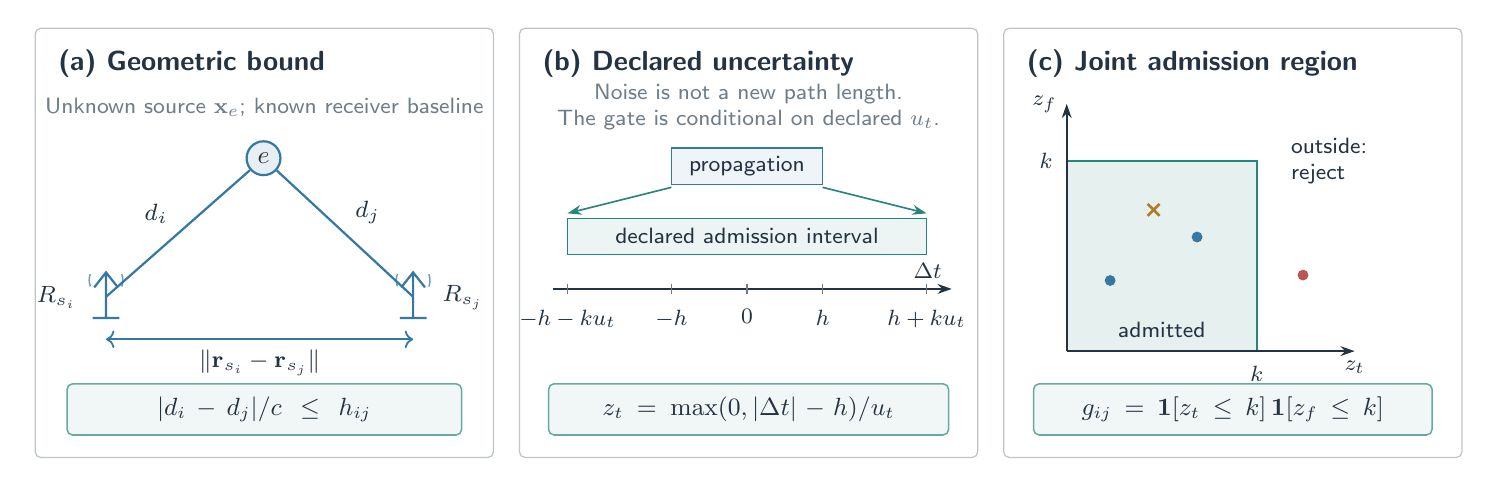
\begin{tikzpicture}[x=1cm,y=1cm]
\draw[panel] (0,0) rectangle ++(5.82,5.45);
\node[heading] at (0.17,5.3) {(a) Geometric bound};
\draw[panel] (6.15,0) rectangle ++(5.82,5.45);
\node[heading] at (6.32,5.3) {(b) Declared uncertainty};
\draw[panel] (12.3,0) rectangle ++(5.82,5.45);
\node[heading] at (12.47,5.3) {(c) Joint admission region};

\node[dot,fill=physical!12] (src) at (2.9,3.8) {$e$};
\pic at (.9,1.77) {receiver};\pic at (4.8,1.77) {receiver};
\coordinate (ri) at (.9,2.04);\coordinate (rj) at (4.8,2.04);
\draw[link] (src)--node[above left,smalllabel] {$d_i$} (ri);
\draw[link] (src)--node[above right,smalllabel] {$d_j$} (rj);
\draw[<->,physical,line width=.65pt] (.9,1.5)--node[below,smalllabel] {$\|\mathbf r_{s_i}-\mathbf r_{s_j}\|$} (4.8,1.5);
\node[smalllabel,anchor=east] at (.64,2.03) {$R_{s_i}$};
\node[smalllabel,anchor=west] at (5.05,2.03) {$R_{s_j}$};
\node[gate,text width=4.8cm,minimum height=.65cm] at (2.91,.61)
 {$|d_i-d_j|/c\leq h_{ij}$};
\node[tinylabel,text=muted] at (2.91,4.45) {Unknown source $\mathbf x_e$; known receiver baseline};

\draw[draw=physical,fill=physical!8] (8.08,3.47) rectangle (10.0,3.93);
\node[tinylabel] at (9.04,3.7) {propagation};
\draw[draw=feasible,fill=feasible!8] (6.76,2.58) rectangle (11.32,3.04);
\node[tinylabel] at (9.04,2.81) {declared admission interval};
\draw[edge] (6.57,2.14)--(11.64,2.14) node[above left,tinylabel] {$\Delta t$};
\foreach \xx/\lab in {6.76/{-h-ku_t},8.08/{-h},9.04/{0},10.0/{h},11.32/{h+ku_t}} {
  \draw[muted,line width=.5pt] (\xx,2.08)--(\xx,2.2);
  \node[tinylabel,anchor=north] at (\xx,2.0) {$\lab$};
}
\draw[edge,feasible] (8.08,3.43)--(6.76,3.10);
\draw[edge,feasible] (10,3.43)--(11.32,3.10);
\node[gate,text width=4.87cm,minimum height=.65cm] at (9.06,.61)
 {$z_t=\max(0,|\Delta t|-h)/u_t$};
\node[tinylabel,text=muted,align=center] at (9.06,4.45) {Noise is not a new path length.\\The gate is conditional on declared $u_t$.};

\begin{scope}[shift={(13.10,1.35)},x=.69cm,y=.69cm]
  \fill[feasible!12] (0,0) rectangle (3.5,3.5);
  \draw[feasible,line width=.8pt] (0,3.5)--(3.5,3.5)--(3.5,0);
  \draw[edge] (0,0)--(5.3,0) node[below,tinylabel] {$z_t$};
  \draw[edge] (0,0)--(0,4.55) node[left,tinylabel] {$z_f$};
  \node[tinylabel,anchor=north] at (3.5,-.09) {$k$};
  \node[tinylabel,anchor=east] at (-.08,3.5) {$k$};
  \fill[physical] (.8,1.3) circle (.10);\fill[physical] (2.4,2.1) circle (.10);
  \draw[semantic,line width=1pt] (1.6,2.6) ++(-.11,-.11)--++(.22,.22) ++(-.22,0)--++(.22,-.22);
  \fill[fault] (4.35,1.4) circle (.10);
  \node[tinylabel,align=left,anchor=west] at (3.95,3.5) {outside:\\reject};
  \node[tinylabel] at (1.75,.4) {admitted};
\end{scope}
\node[gate,text width=4.85cm,minimum height=.65cm] at (15.21,.61)
 {$g_{ij}=\mathbf 1[z_t\leq k]\,\mathbf 1[z_f\leq k]$};
\end{tikzpicture}
\end{document}
